\documentclass{article}
\usepackage{authblk}
\usepackage{graphicx}
\usepackage{placeins}
\usepackage{booktabs}

\title{Weakly Supervised Software Entity Recognition}
\author[1]{Dumitrescul Eduard-Valentin}
\author[2]{Huțanu Eusebiu-Ciprian}
\author[3]{Mircea Andrei-Răzvan}
\author[4]{Păpușoi Rareș}
\affil{University of Bucharest}



\begin{document}

\maketitle

\begin{abstract}

\end{abstract}


\section{Introduction}
The quality and quantity of data is the single most important factor when 
developing and using a state-of-the-art Large Language Model. One of the most 
popular use-cases of such models is writing code based on a prompt. During 
both training and inference, the LLM has access to enormous datasets containing
code examples, which it uses to build upon and answer. We believe that adding 
the ability to filter and group this data can provide a significant increase in 
the quality of the responses and the generated code.

This project aims to develop a Weakly Supervised Software Entity Recognition (SER)
system that is trained using automatically annotated data. The goal is to bypass
the need for expensive manual labeling and make use of Transformer architectures
to build a system that can identify important entities within source code and 
technical documentation.

\subsection{Background}
\textbf{Named Entity Recognition} is a Natural Language Processing task that 
aims to identify specific entities \textemdash like names, dates and places 
\textemdash in bodies of text. The challenge of this project is to identify a 
set of predefined entities in text that does not possess classic linguistic 
features.

\textbf{Manual annotation} is the standard for most machine learning projects.
It has the ability to generate high-quality of data, but requires
large teams of specialized people. Specifically for SER, the annotation process
requires domain expertise (software engineers), which makes the task incredibly
expensive. Another issue is the constant changing of the existent programming 
languages and the creation of new ones that created the need of a constantly 
evolving dataset.

\textbf{Weakly Supervision} is the solution we propose for this problem. It 
replaces the manual effort of manually annotating data with training the model 
on noisy, imperfect of incomplete data. However, by defining rules for annotating 
the data, it is possible to generate large amounts of annotated data that make 
up for the lower quality if the labels. This approach is reusable and easily 
extensible.

\textbf{Transformer architectures} are very effective for SER because of their 
ability to understant large amounts of data. Specifically, \textbf{CodeBERT}, 
which is pretrained in such a way that it understand both natural language and
programming language.

\section{Methodology}
\subsection{Target Entities}
This SER system focuses on a set of high-value 4 core entities found in the
majority of programming languages.

\begin{itemize}
    \item \textbf{LIBRARY}: Software packages or modules (e.g. \textit{numpy})
    \item \textbf{FUNCTION\_METHOD}: A function or a method name (e.g. \textit{sum()})
    \item \textbf{CLASS\_NAME}: A class definition or its usage (e.g \textit{DataLoader})
    \item \textbf{FILE\_PATH}: Relative or absolute file paths(e.g. \textit{/etc/config})
\end{itemize}

\subsection{Data Gathering}
\FloatBarrier
The principal data source is an archive of \textbf{Stack Overflow posts, votes,  
tags and badges}. Question bodies were extracted for both \textbf{python}
and \textbf{javascript} programming languages, based on their tags. The two 
lanugages were chosen because of their popularity, the vast amount of data 
available for both of them and the significant syntactic difference between them.
For consistency, only questions containing between 800 and 1000 words were selected.

\begin{figure}
    \centering
    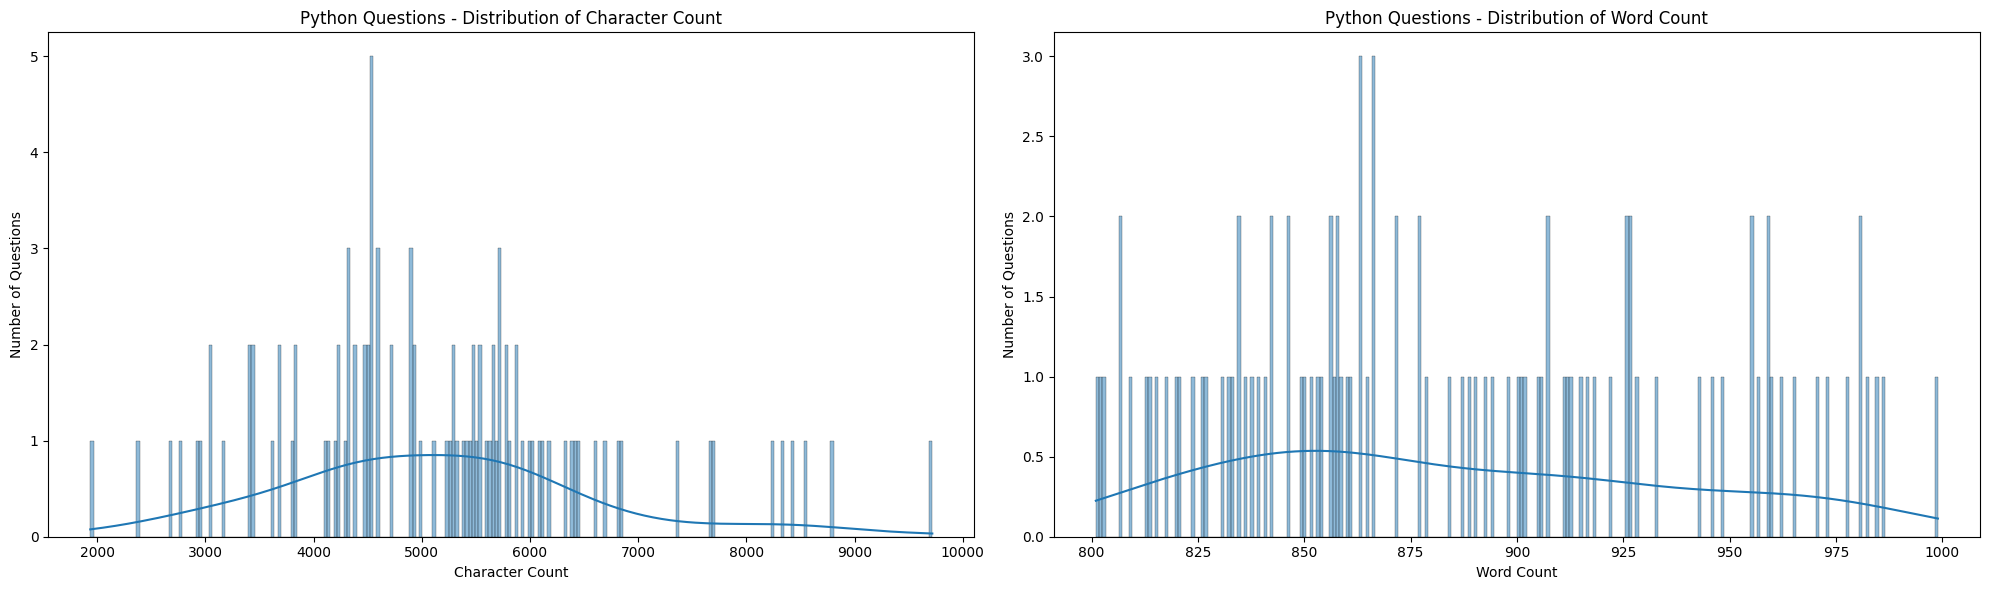
\includegraphics[width=0.8\textwidth]{images/ch-word-count-py.png}
    \caption{The distribution of character and word count based on 100 Python questions}
\end{figure}

\begin{figure}
    \centering
    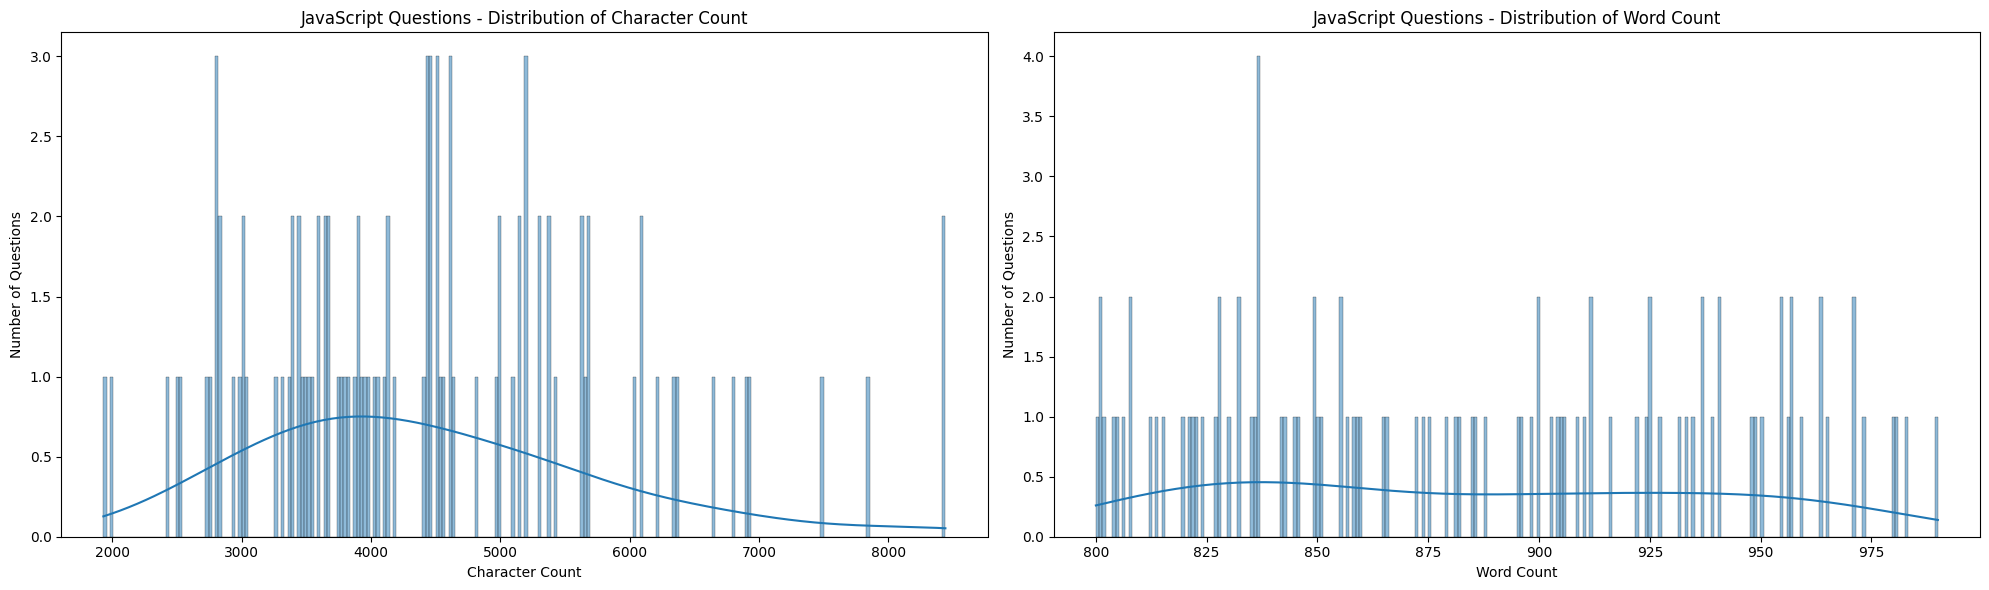
\includegraphics[width=0.8\textwidth]{images/ch-word-count-js.png}
    \caption{The distribution of character and word count based on 100 JavaScript questions}
\end{figure}

\FloatBarrier

\subsection{Data Preprocessing}
The body of each questions contains HTML tags and code snippets. To prepare the
data for SER, the code blocks were extracted and concatenated based on the HTML tags present. Only the code blocks have been selected because they contain the highest 
density of the defined entities. Both Pythona dn JavaScript data was preprocessed
in this way.

\subsection{Annotation Process}
A series of \textbf{Labeling Functions} were developed for labeling 
the Python data for all 4 entities: LIBRARY, FUNCTION\_METHOD, CLASS and FILEPATH.
The LFs were built using a combination and regex and predefined keywords.

For \textbf{Library extraction}, three distinct LFs identify import patterns, covering:
direct import (e.g. \textit{import os})
aliased imports (e.g. \textit{import pandas as pd})
partial imports (e.g. \textit{from math import sqrt})

For \textbf{Function and Method identification} definitions  (using \textit{def} 
keyword) and method and function invocation were targeted (e.g. \textit{object.method()}).

\textbf{Class detection} is based on detecting class definition and instantiation patterns.
To improve precision, the LFs look for PascalCase identifiers.

\textbf{Filepath identification} uses LFs that search for Unix-style paths (e.g. \textit{/etc/config}), Windows-style
paths (e.g. \textit{C:/Python}) and standalone filenames (e.g. \textit{config.json})

\subsection{Tokenization}
\FloatBarrier
In order to prepare the data for feeding it into SER models, the \textit{codebert-base} tokenizer was 
used on the preprocessed code blocks, creating the embeddings for the test. Then, 
the token-level labels (\textit{IOB2 tags}) for each entity were generated.

A total of 9 tags were used: \textit{O, B-LIBRARY, I-LIBRARY, B-CLASS\_NAME, I-CLASS\_NAME, B-FILE\_PATH, I-FILE\_PATH, B-FUNCTION\_METHOD, I-FUNCTION\_METHOD}.

\begin{table}[ht]
    \centering
    \resizebox{\textwidth}{!}{%
    \begin{tabular}{@{}rccccccccccccc@{}}
    \toprule
    \textbf{Index} & 0 & 1 & 2 & 3 & 4 & 5 & 6 & 7 & 8 & 9 & 10 & 11 & 12 \\ \midrule
    \textbf{Token} & \texttt{<s>} & \texttt{import} & \texttt{Ġc} & \texttt{Pick} & \texttt{le} & \texttt{Ġas} & \texttt{Ġpick} & \texttt{le} & \texttt{Ġ\#} & \texttt{orig} & \texttt{inally} & \texttt{Ġpick} & \texttt{le} \\
    \textbf{Label} & O & O & B-LIB & B-LIB & I-LIB & O & B-LIB & I-LIB & O & O & O & B-LIB & I-LIB \\ \bottomrule
    \end{tabular}%
    }
    \caption{Tokenization and IOB Tagging Output}
\end{table}
\FloatBarrier

\section{Experimental Setup}
\subsection{CodeBERT}
\subsection{Custom Model}

\section{Results and Evaluation}
\section{Discussion}

\section{Conclusion}

\end{document}